\chapter{Distributed Computing}\label{chap:dcap} 
As described in the previous chapter, we planned on creating a large number of predictive models. In order to scale such a large number of experiments, we needed a parallelization framework to accomplish machine learning at scale, utilizing the computing power of CSAIL's openstack cloud.

In order to accomplish this, we modified a parallelization framework called DCAP to run our experiments. DCAP is a master-slave architected system built in the ALFA group that allows a user to manage the execution list of computational jobs \cite{alex}. The list of jobs is called a taskfile. DCAP takes a taskfile and launches a server to which clients can connect. Each time a client connects, the DCAP server sends it a job (including a config file) from the taskfile. The client executes the job and sends the result back to the master. This repeats until there are no more jobs to accomplish. Figure \ref{fig:dcap} shows the flow of jobs.

\begin{figure}[ht!]
  \caption{The client-server architecture of DCAP. It is used to parallelize the model prediction process.}\label{fig:dcap}
  \centering
    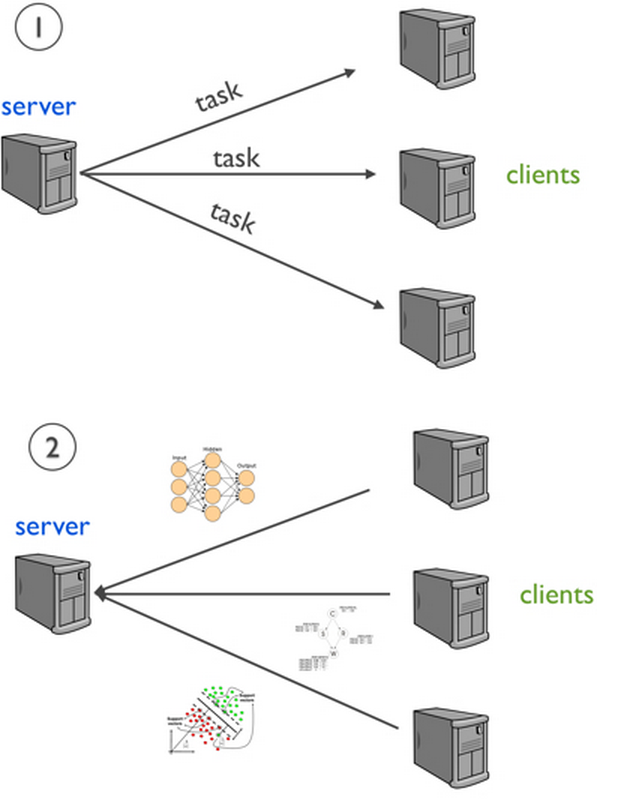
\includegraphics[width=1.0\textwidth]{figures/dcap.png}
\end{figure}

We used DCAP to run a large suite of jobs on the cloud. This involved generating taskfiles and config files for each experiment. In addition, we created scripts to launch clients that will automatically connect to a server. We employed the eucalyptus API to manage cloud nodes. Additionally, we created image snapshots containing the datasets and the model creation code to run. The scripts instructed openstack to launch nodes using the images containing the necessary libraries and datasets. Next, the clients would automatically connect to the server and run jobs until all the tasks were finished.

In particular, we used DCAP to run all HMM and logistic regression on HMM state jobs. These model variants are by far the most computational intensive. This included several job launches as we progressively fine tuned our models. Each run included additional modifications, such as training 10 HMMs per experiment to avoid local maxima, and using feature-sets with dimensionality reduction through principal component analysis. Usually, the runs include 84 jobs. This included both types of models, all 4 cohorts, and 14 different hidden variable supports. Due to computational complexity of the algorithms, the final run included 84 jobs, used 22 12-core machines and took around 1 week to finish. Running experiments at this scale would not have been possible if it were not for cloud computing. Using DCAP to do so saved a lot of micro-managing, as everything was ran through scripts automatically.